\section{Latent Alignment Model for Lexical-Anchoring Graph-based Parsing}
\label{sec:lex-phr:graph-based}

In this section, we will introduce the two-stage framework for parsing
the DM, PSD, and AMR graphs~\S\ref{sec:lex-phr:two-stage}. Then we
resolve the alignment problem with a latent alignment model~\S\ref{sec:lex-phr:latent-alignment}

\subsection{Two-stage Graph-Based Parsing}
\label{sec:lex-phr:two-stage}

Before formulating the graph-based model into a probabilistic model as
Equation \ref{eq:graph_prob}, we denote some notations: $C$, $R$ are
sets of concepts (nodes) and relations (edges) in the graph, and $w$
is a sequence of tokens.  $a \in {\mathbb{Z}}^m$ as the alignment
matrix, each $a_{i}$ is the index of aligned token where $i$th node
aligned to. When modeling the negative log likelihood loss~(NLL), with
independence assumption between each node and edge, we decompose it
into node- and edge-identification pipelines.

\begin{equation}
  \label{eq:graph_prob}
\begin{aligned} \smaller[2]
 & NLL(P(C,R \mid w)) \\
 & = - \log(P(C,R \mid w)) \\
 & = - \log(\sum_{a}{P(a) P(C,R \mid w,a)}) \\
 & = - \log\left(\sum_{a}P(a) P(R\mid w,a,C) P(C \mid w, a)\right) \\
 & = - \log\left(\sum_{a}P(a) \prod_{i}^{m} P(c_{i} \mid h_{a_{i}}) \right. \\
 & \qquad \left.\cdot \prod_{i,j=1}^{m}P(r_{ij} \mid h_{a_{i}}, c_{i}, h_{a_{j}}, c_{j})\right)
\end{aligned}
\end{equation}

In DM, PSD, and AMR, every token will only be aligned once.  Hence, we
train a joint model to maximize the above probability for both node
identification
$P(c_{i} \mid h_{a_{i}})$~\S\ref{sssec:lex-phr:node-indent} and edge
identification
$P(r_{ij} \mid h_{{a_{i}}, c_{i},h_{a_{j}},
  c_{j}})$~\S\ref{sssec:lex-phr:edge-indent}. The alignment
information is mainly used for training. We need to marginalize out
the discrete alignment variable $a$ to jointly learning the parameters
in node identification and relation identification networks. We will
introduce the latent alignment model
in~\autoref{ssec:lex-phr:latent-alignment}. \autoref{fig:graph-based-inference}
summerize the unifed two-stage graph based parsing framework. In the
following subsections, we will explain the framework in more details.

\begin{figure}[h] \centering
  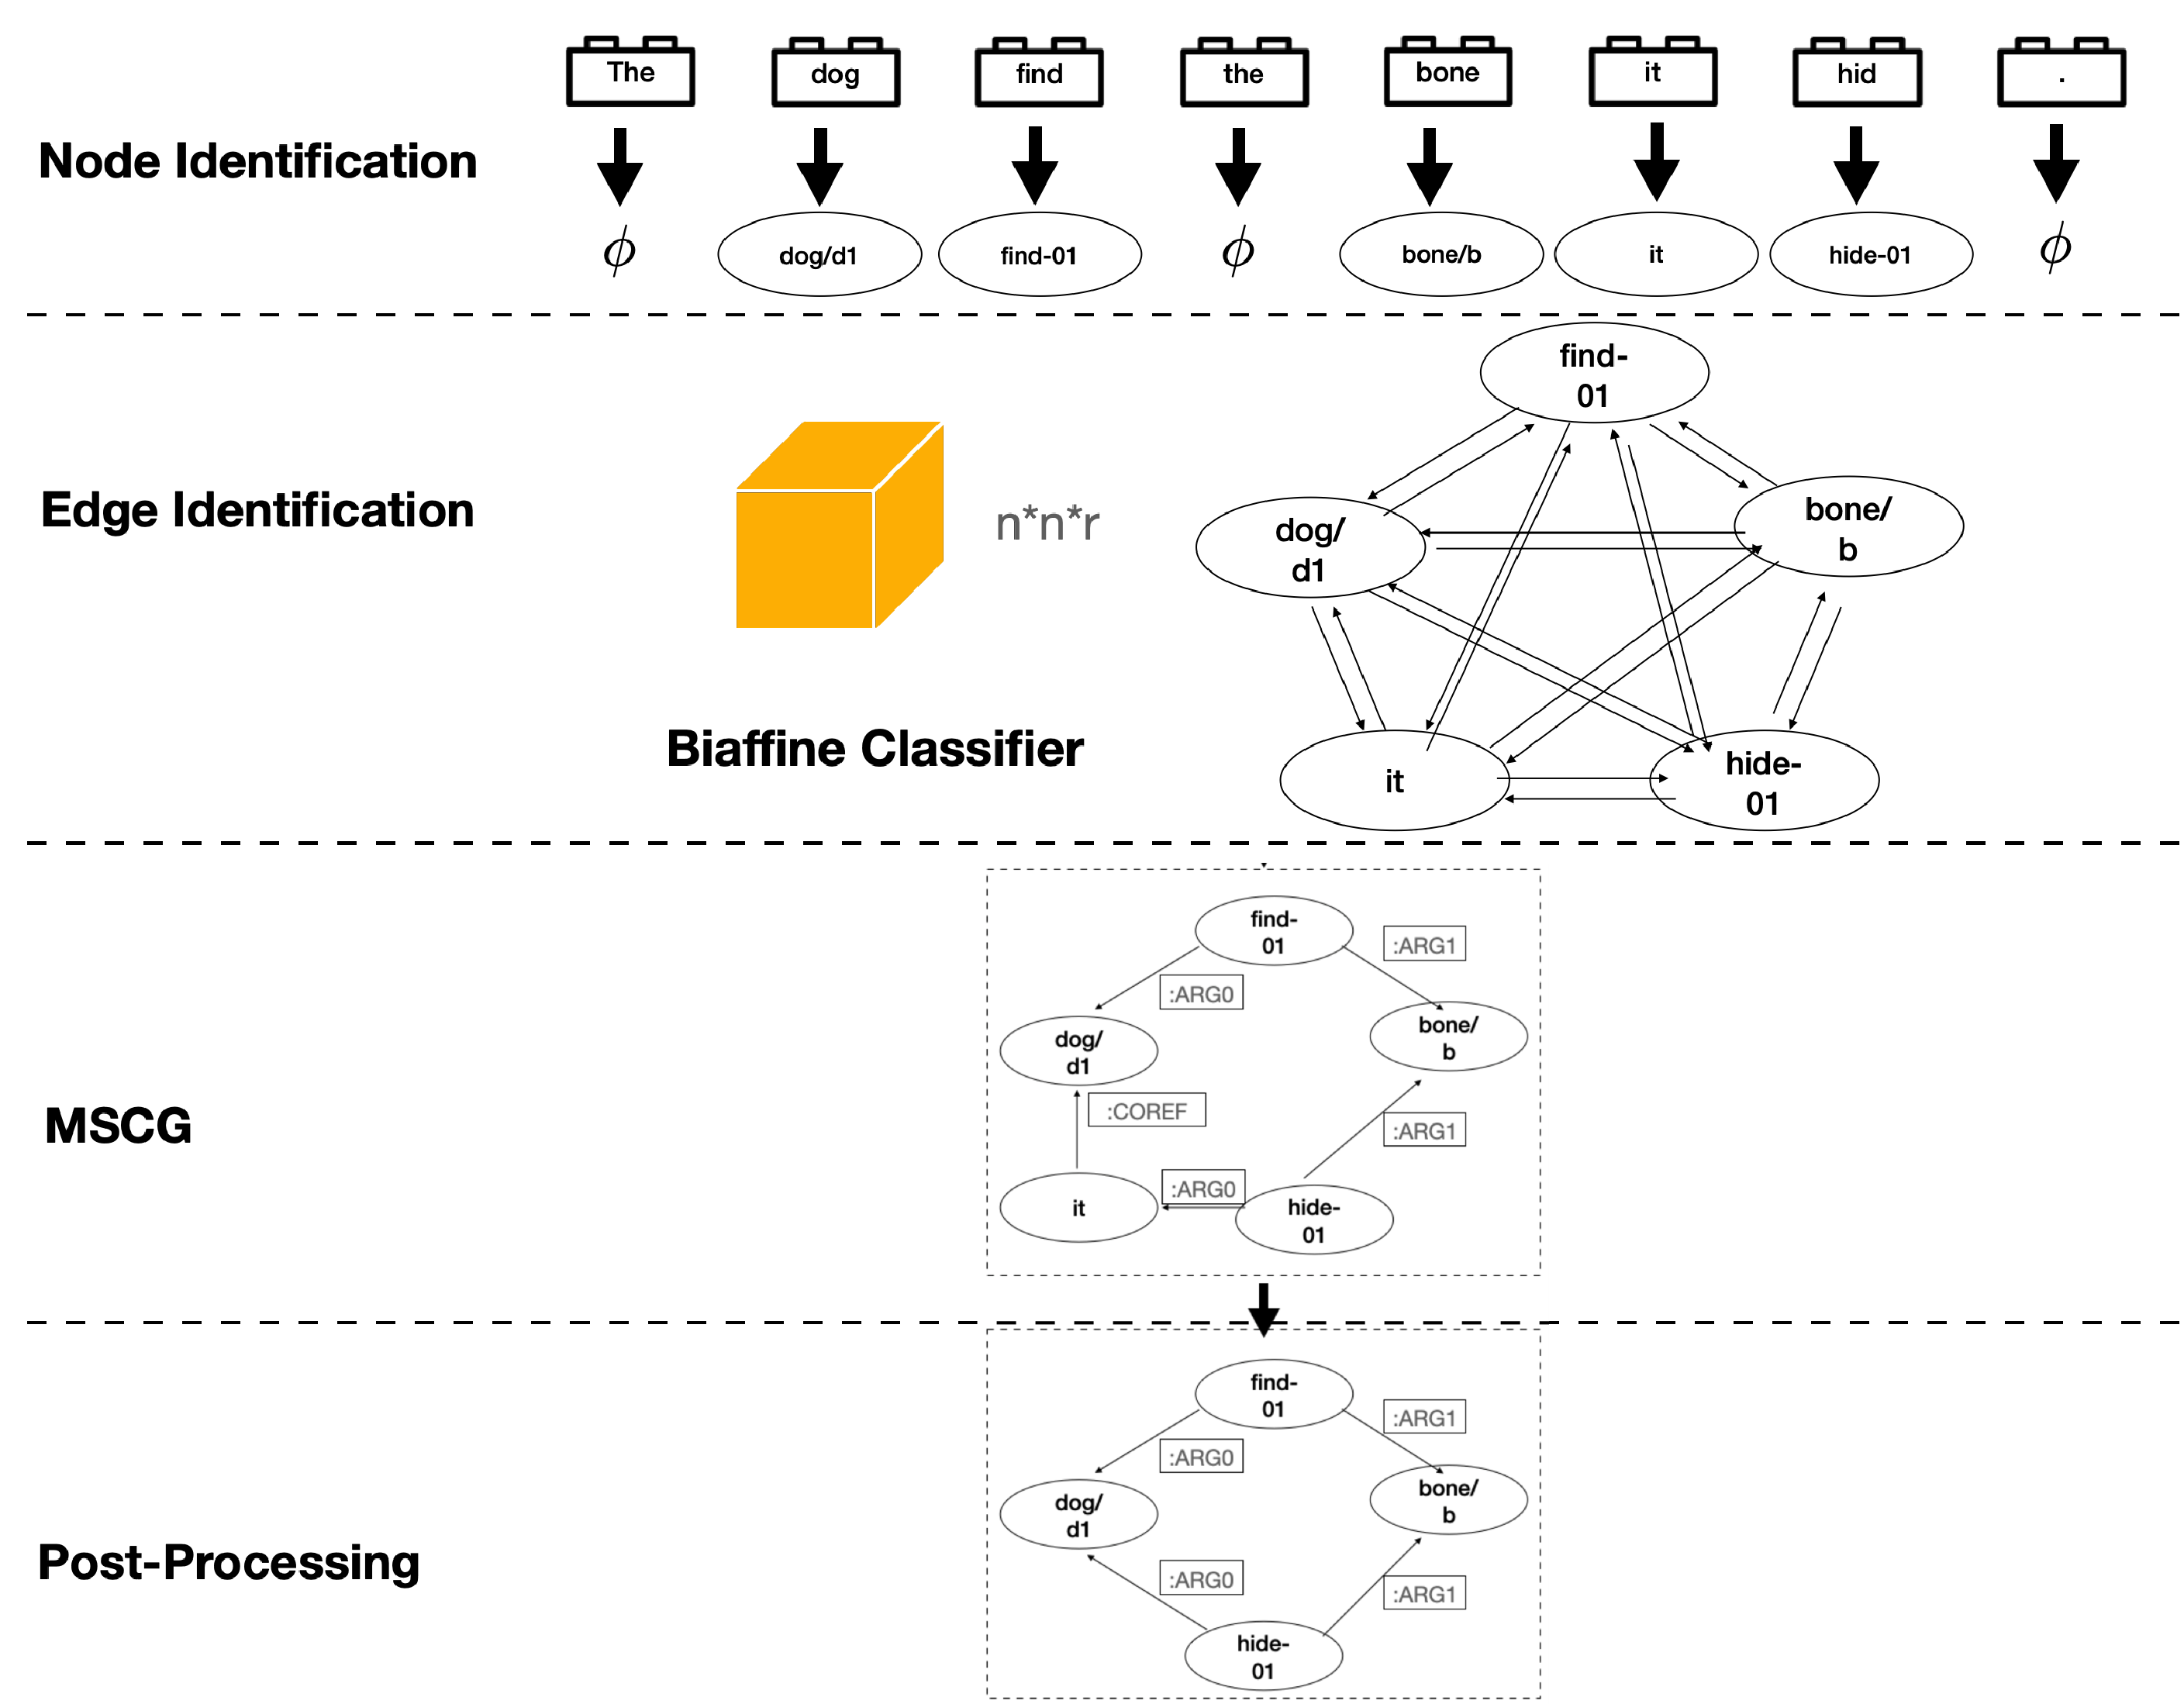
\includegraphics[width=1.00\textwidth]{graph-overview3.pdf}
\caption{\label{fig:graph-based-inference} Architecture of graph-based model and inference, for running exmaple [wsj\#0209013]}
\end{figure}

\subsubsection{Node Identification}
\label{sssec:lex-phr:node-ident}
Node Identification predicts a concept $c$ given a word. A
concept can be either {\it NULL} (when there is no semantic node
anchoring to that word, e.g., the word is dropped), or a node label
(e.g., lemma, sense, POS, name value in AMR, frame value in PSD), or
other node properties. One challenge in node identification is the
data sparsity issue. Many of the labels are from open sets derived
from the input token, e.g., its lemma.  Moreover, some labels are
constrained by a deterministic label set given the word. Hence, we
designed a copy mechanism~\citep{luong2014addressing} in our neural
network architecture to decide whether to copying deterministic label
given a word or estimate a classification probability from a fixed
label set.


\subsubsection{Edge Identification}
\label{sssec:lex-phr:edge-ident}

By assuming the independence of each edge, we model the edges
probabilites independently.  Given two nodes and their underlying
tokens, we predict the edge label as the semantic relation between the
two concepts with a bi-affine classifier~\cite{dozat2016deep}.

\subsubsection{Inference}
\label{sssec:lex-phr:inference}
In our two-stage graph-based parsing, after nodes are identified, edge
identification only output a probility distribution over all the
relations between identified nodes. However, we need to an inference
algorithm to search for the \kw{maximum spanning connected graph} from all
the relations. We use~\citet[MSCG,][]{Flanigan:2014vc} to greedily
select the most valuable edges from the identified nodes and their
relations connecting them. As shown in Figure
\ref{fig:graph-based-inference}, an input sentence goes through
preprocessing, node identification, edge identification, root
identification, and MCSG to generate a final connected graph as
structured output.

\subsection{Latent Alignment Model}
\label{ssec:lex-phr:latent-alignment}

As the two-stage probablistic model shown
in~\autoref{eq:graph_prob_bried}, we need to marginalize all the
alignment information $a$ to learn the above two-stage nerual networks
for node and edge identification. We do the following computing for
explicit and implicit alignments respectively.

\Paragraph{Explicit Alignments} For DM, PSD, with explicit alignments
$a*$, we can simply use $P(a^{*}) = 1.0$ and other alignments
$P(a | a \neq a^{*}) = 0.0 $. In this case, with known alignment
information, we don't need to worry the marginalization problem.

\Paragraph{Implicit Alignments} However, For AMR, without gold
alignments, one requires to compute all the valid alignments and then
condition the node- and edge-identification methods on the alignments.
However, it is computationally intractable to enumerate all
combinatoral values for the discrete alignment variable. Hence, we
estimate the latent alignments via variational inferece, which has
been initialially used in \citet{lyu2018amr}. In the following
section, we firstly introduce the details of latent alignment model
via continuous relaxiation~\S\ref{sssec:lex-phr:alignment-relax} and
then we descibe the details of variational
inference~\S\ref{sssec:lex-phr:gumble-sinkhorn}, and we propose a
error fix for computing KL-divergence with implicit Gumbel-Sinkhorn
distribution.

\begin{equation}
  \label{eq:graph_prob_brief}
\begin{aligned} \smaller[2]
 & NLL(P(C,R \mid w)) \\
 & = - \log\left(\sum_{a}P(a) \prod_{i}^{m} P(c_{i} \mid h_{a_{i}}) \right. \\
 & \qquad \left.\cdot \prod_{i,j=1}^{m}P(r_{ij} \mid h_{a_{i}}, c_{i}, h_{a_{j}}, c_{j})\right)
\end{aligned}
\end{equation}

\subsubsection{Continuous Relaxation for Discrete Alignments}
\label{sssec:lex-phr:alignment-relax}

\begin{equation}
 \label{eq:elbo}
\begin{aligned} \smaller[2]
  & \log(P(C,R \mid w)) \geq \\
  & E_{Q}[\log(P_{\theta}(c\mid w,a) P_{\Phi}(R\mid w,a,c))] \\
  & - \kld{Q_{\Psi}(a\mid c, R,w)}{P(a)}
\end{aligned}
\end{equation}

\subsubsection{VAE, Perturb-and-Map, Gumble Sinkhorn}
\label{sssec:lex-phr:gumble-sinkhorn}
\begin{itemize}
\item Applying variational inference to reduce it into
  Evidence Lower Bound~\cite[ELBO,][]{kingma2013auto}
\item The denominator $Z_{\Psi}$ in Q can be estimated by Perturb-and-Max(MAP)~\cite{papandreouperturb}
\begin{equation}
  \label{eq:posterior_prob}
\begin{aligned} \smaller[2]
Q_{\Psi}(a\mid c, R,w)= \frac{\exp(\sum_{i=1}^{n} \phi(g_{i}, h_{a_{i}}))} {Z_{\Psi}(c,w)}
\end{aligned}
\end{equation}
Where $\phi(g_{i}, h_{a_{i}})$ score each alignment link between node i and the corresponding words,
$g_{i}$ is node encoding, and $h_{a_{i}}$ is encoding for the aligned token.

\item Discrete \texttt{argmax} of a permutation can be estimated by
  Gumbel-Softmax Sinkhorn Networks \cite{mena2018learning, lyu2018amr}
\end{itemize}

%%% Local Variables:
%%% mode: latex
%%% TeX-master: "../../thesis-main.ltx"
%%% End:
